\documentclass{article}
\usepackage[margin=1in]{geometry}
\usepackage{amsmath}
\usepackage{amssymb}
\usepackage{graphicx}
\usepackage{caption}
\usepackage{lipsum}


\begin{document}

\title{A Sample Manuscript with a Clean Workflow}
\author{Jacob Jameson}

\maketitle

\section{Introduction}

This is a simple example of a \LaTeX\ document. Here is an equation:

\begin{equation}
    e^{i\pi} + 1 = 0
\end{equation}

\lipsum[1]



\begin{figure}[h!]
    \centering
    \caption{Main caption of the figure.}
    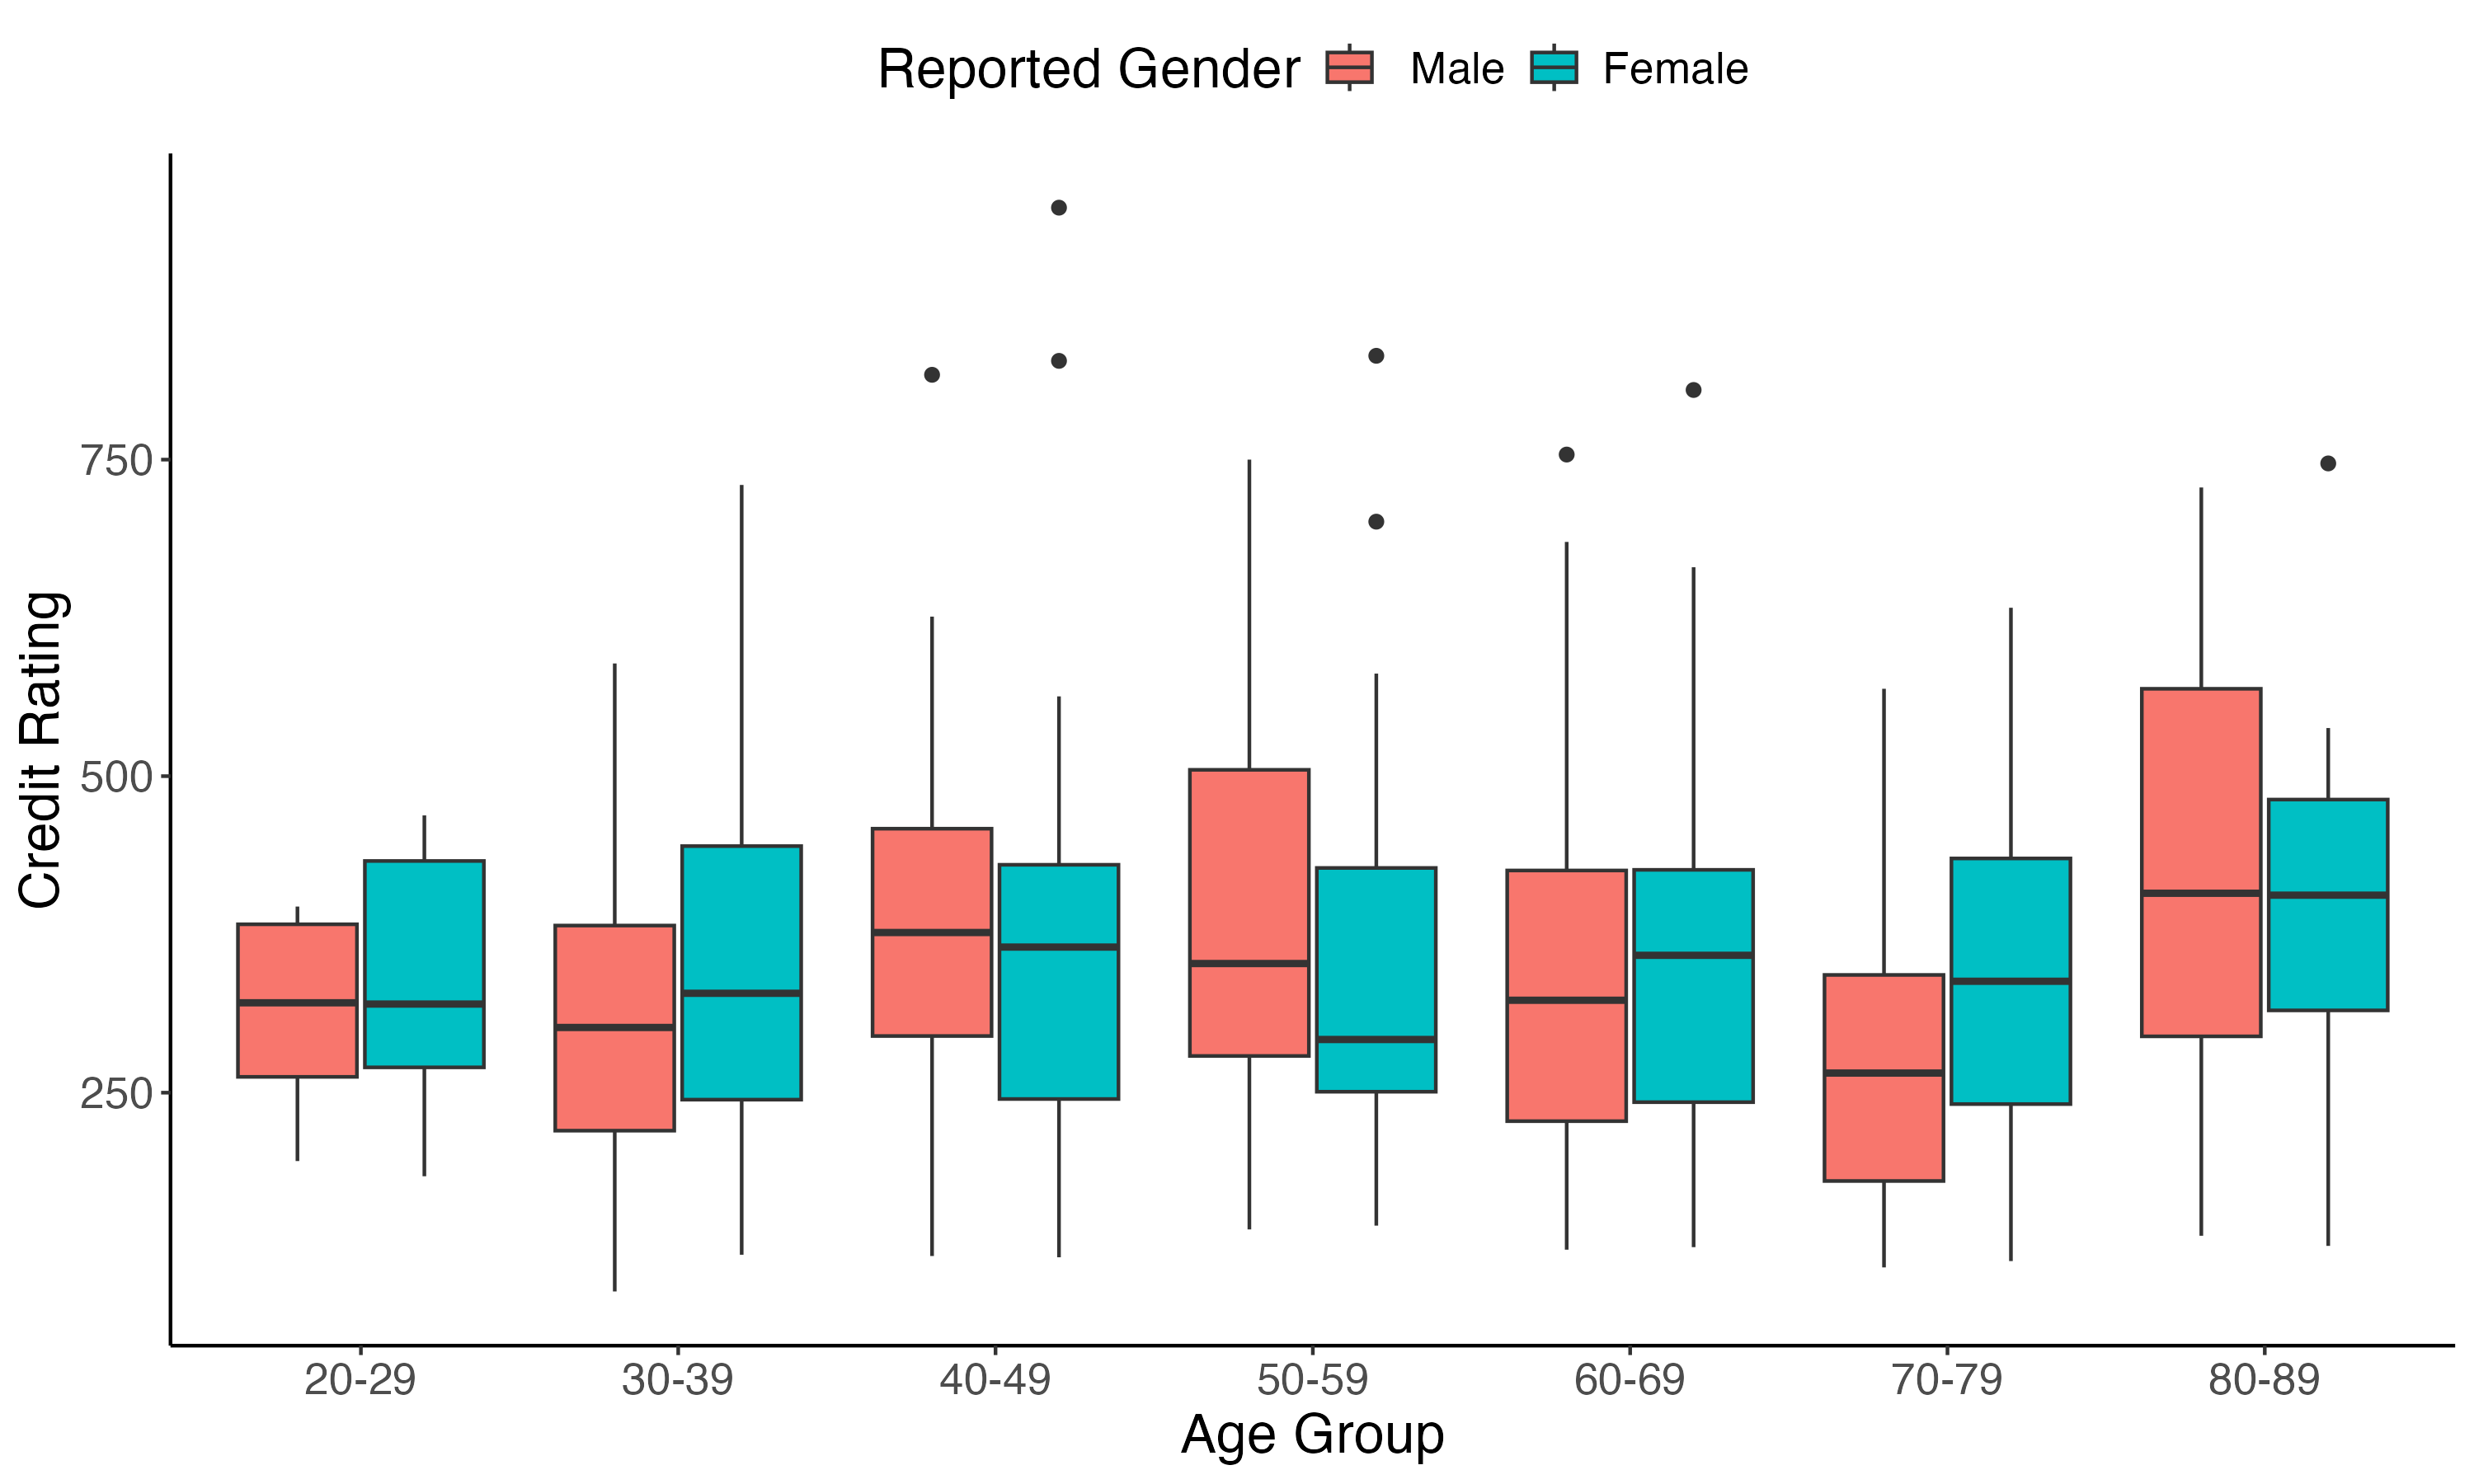
\includegraphics[width=0.8\textwidth]{outputs/figures/fig_1.png}
    \captionsetup{justification=centering, font=small} 
    \caption*{Note: This is an additional note below the main caption.}
    \label{fig:fig_1}
\end{figure}

\lipsum[2]

\section{Results}

\lipsum[3]


% Table created by stargazer v.5.2.3 by Marek Hlavac, Social Policy Institute. E-mail: marek.hlavac at gmail.com
% Date and time: Sat, Oct 26, 2024 - 13:42:30
\begin{table}[!htbp] \centering 
  \caption{Regression Models} 
  \label{} 
\begin{tabular}{@{\extracolsep{5pt}}lccc} 
\\[-1.8ex]\hline 
\hline \\[-1.8ex] 
\\[-1.8ex] & \multicolumn{3}{c}{Credit Rating} \\ 
 & Model 1 & Model 2 & Model 3 \\ 
\\[-1.8ex] & (1) & (2) & (3)\\ 
\hline \\[-1.8ex] 
 Age & 0.925$^{**}$ & 0.020 & 0.002 \\ 
  & (0.448) & (0.036) & (0.030) \\ 
  & & & \\ 
 Female & 2.619 & $-$0.128 & 0.114 \\ 
  & (15.438) & (1.228) & (1.029) \\ 
  & & & \\ 
 Income &  & 0.018 & 0.033 \\ 
  &  & (0.029) & (0.024) \\ 
  & & & \\ 
 Credit Limit &  & 0.067$^{***}$ & 0.066$^{***}$ \\ 
  &  & (0.0004) & (0.0004) \\ 
  & & & \\ 
 Number of Cards &  &  & 4.893$^{***}$ \\ 
  &  &  & (0.376) \\ 
  & & & \\ 
 Student &  &  & 2.527 \\ 
  &  &  & (1.716) \\ 
  & & & \\ 
 Constant & 302.089$^{***}$ & 37.738$^{***}$ & 24.137$^{***}$ \\ 
  & (27.258) & (2.492) & (2.333) \\ 
  & & & \\ 
\textit{N} & 400 & 400 & 400 \\ 
R$^{2}$ & 0.011 & 0.994 & 0.996 \\ 
Adjusted R$^{2}$ & 0.006 & 0.994 & 0.996 \\ 
Residual Std. Error & 154.280 (df = 397) & 12.262 (df = 395) & 10.260 (df = 393) \\ 
F Statistic & 2.150 (df = 2; 397) & 15,783.710$^{***}$ (df = 4; 395) & 15,056.920$^{***}$ (df = 6; 393) \\ 
\hline 
\hline \\[-1.8ex] 
\textit{Notes:} & \multicolumn{3}{r}{$^{***}$Significant at the 1 percent level.} \\ 
 & \multicolumn{3}{r}{$^{**}$Significant at the 5 percent level.} \\ 
 & \multicolumn{3}{r}{$^{*}$Significant at the 10 percent level.} \\ 
\end{tabular} 
\end{table} 



\section{Conclusion}

\lipsum[4-6]

\end{document}
